\documentclass{jknotes}
\usepackage{joshkirklin,pgfplots}

\usepackage{xcolor}
\usepackage{wrapfig}
\usepackage{placeins}
\newcommand{\VL}[1]{\mathbf{#1}}
\newcommand{\Ro}{Ro}
\newcommand{\Ek}{E}
\newcommand{\vare}{\varepsilon}

\usepackage{tikz}
\usepackage{tikz-3dplot}
\usepackage{pgfplots}
\pgfplotsset{compat = 1.3}
\usetikzlibrary{arrows}
\usetikzlibrary{calc}

\tikzset{
    partial ellipse/.style args={#1:#2:#3}{
        insert path={+ (#1:#3) arc (#1:#2:#3)}
    }
}

\begin{document}

\institution{Cambridge Part III Maths}
\title{Fluid Dynamics of Climate}
\lecturer{John Taylor \& Peter Haynes}
\notetaker{Charles Powell}
\date{Michaelmas 2020}

\maketitle
\suggestionsspiel
\tableofcontents

\lecture{12/10/20}
\section{Fluid motion in a rotating reference frame}
In a non-rotating frame, the \emph{Navier-Stokes} equations are
\begin{equation}
	\rho \frac{\diffD \bm{u}}{\diffD t} = -\nabla p - \rho \nabla \phi + \rho
	\bm{F}
	\label{ns}
\end{equation}

The body forces are assumed to be conservative with potential $\phi$, e.g.
$\phi = gz$ for gravitational force. $\bm{F}$ is the frictional force.

Consider a reference frame rotating about the $z$-axis with constant angular
velocity $\bm{\Omega}$. Axes in the inertial frame are denoted with a
subscript $_I$ and axes in the rotating frame are denoted with a subscript
$_R$.

\begin{center}
\newcommand{\TikzInnerSep}{0.33mm}

% Define new arc command
% Syntax: [draw options] (center) (initial angle:final angle:radius)
% https://tex.stackexchange.com/a/66220
\def\centerarc[#1](#2)(#3:#4:#5){%
	\draw [#1] ($(#2)+({#5*cos(#3)}, {#5*sin(#3)})$) arc (#3:#4:#5)%
}

% Redefine the rotation sequence for the tikz3d-plot to Euler-Angles:
% z-x-z with alpha-beta-gamma (psi-theta-phi)
% https://tex.stackexchange.com/q/118069/98906
\newcommand{\tdseteulerzxz}{%
	\renewcommand{\tdplotcalctransformrotmain}{%
		%
		% Determine the sin and cos of the specified angle in degrees
		% \tdplotsinandcos{sin}{cos}{theta}
		% - #1: Returns sin(#3)
		% - #2: Returns cos(#3)
		% - #3: User-specified angle theta
		\tdplotsinandcos{\sinalpha}{\cosalpha}{\tdplotalpha} 
		\tdplotsinandcos{\sinbeta}{\cosbeta}{\tdplotbeta}
		\tdplotsinandcos{\singamma}{\cosgamma}{\tdplotgamma}
		%
		% Define trigonometric abbreviations
		%
		\tdplotmult{\sasb}{\sinalpha}{\sinbeta}
		\tdplotmult{\sacb}{\sinalpha}{\cosbeta}
		\tdplotmult{\sacbsg}{\sacb}{\singamma}
		\tdplotmult{\sacbcg}{\sacb}{\cosgamma}
		\tdplotmult{\sasg}{\sinalpha}{\singamma}
		\tdplotmult{\sacg}{\sinalpha}{\cosgamma}
		%
		\tdplotmult{\sbsg}{\sinbeta}{\singamma}
		\tdplotmult{\sbcg}{\sinbeta}{\cosgamma}
		%
		\tdplotmult{\casb}{\cosalpha}{\sinbeta}
		\tdplotmult{\cacb}{\cosalpha}{\cosbeta}
		\tdplotmult{\cacbsg}{\cacb}{\singamma}
		\tdplotmult{\cacbcg}{\cacb}{\cosgamma}
		\tdplotmult{\casg}{\cosalpha}{\singamma}
		\tdplotmult{\cacg}{\cosalpha}{\cosgamma}
		%
		% Define the entries for the rotation matrix from the B-System to the I-System
		% This is A_IB = (A_BI)^T
		%
		\pgfmathsetmacro{\raaeul}{+\cacg - \sacbsg}
		\pgfmathsetmacro{\rabeul}{-\casg - \sacbcg}
		\pgfmathsetmacro{\raceul}{+\sasb}
		%
		\pgfmathsetmacro{\rbaeul}{+\sacg + \cacbsg}
		\pgfmathsetmacro{\rbbeul}{-\sasg + \cacbcg}
		\pgfmathsetmacro{\rbceul}{-\casb}
		%
		\pgfmathsetmacro{\rcaeul}{+\sbsg}
		\pgfmathsetmacro{\rcbeul}{+\sbcg}
		\pgfmathsetmacro{\rcceul}{+\cosbeta}
		%
	}
}

% Redefine the rotation sequence for the tikz3d-plot to Cardan-Angles:
% x-y-z with alpha-beta-gamma
% https://tex.stackexchange.com/q/118069/98906
\newcommand{\tdsetcardanxyz}{%
	\renewcommand{\tdplotcalctransformrotmain}{%
		%
		% Determine the sin and cos of the specified angle in degrees
		% \tdplotsinandcos{sin}{cos}{theta}
		% - #1: Returns sin(#3)
		% - #2: Returns cos(#3)
		% - #3: User-specified angle theta
		\tdplotsinandcos{\sinalpha}{\cosalpha}{\tdplotalpha} 
		\tdplotsinandcos{\sinbeta}{\cosbeta}{\tdplotbeta}
		\tdplotsinandcos{\singamma}{\cosgamma}{\tdplotgamma}
		%
		% Define trigonometric abbreviations
		%
		\tdplotmult{\sasb}{\sinalpha}{\sinbeta}
		\tdplotmult{\sasbsg}{\sasb}{\singamma}
		\tdplotmult{\sasbcg}{\sasb}{\cosgamma}
		%
		\tdplotmult{\sacb}{\sinalpha}{\cosbeta}
		\tdplotmult{\sasg}{\sinalpha}{\singamma}
		\tdplotmult{\sacg}{\sinalpha}{\cosgamma}
		%
		\tdplotmult{\casb}{\cosalpha}{\sinbeta}
		\tdplotmult{\casbsg}{\casb}{\singamma}
		\tdplotmult{\casbcg}{\casb}{\cosgamma}
		%
		\tdplotmult{\cacb}{\cosalpha}{\cosbeta}
		\tdplotmult{\casg}{\cosalpha}{\singamma}
		\tdplotmult{\cacg}{\cosalpha}{\cosgamma}
		\tdplotmult{\cbsg}{\cosbeta}{\singamma}
		\tdplotmult{\cbcg}{\cosbeta}{\cosgamma}
		%
		% Define the entries for the rotation matrix from the B-System to the I-System
		% This is A_IB = (A_BI)^T
		%
		\pgfmathsetmacro{\raaeul}{+\cbcg}
		\pgfmathsetmacro{\rabeul}{-\cbsg}
		\pgfmathsetmacro{\raceul}{+\sinbeta}
		%
		\pgfmathsetmacro{\rbaeul}{+\casg + \sasbcg}
		\pgfmathsetmacro{\rbbeul}{+\cacg - \sasbsg}
		\pgfmathsetmacro{\rbceul}{-\sacb}
		%
		\pgfmathsetmacro{\rcaeul}{+\sasg - \casbcg}
		\pgfmathsetmacro{\rcbeul}{+\sacg + \casbsg}
		\pgfmathsetmacro{\rcceul}{+\cacb}
		%
	}
}

% Plot display orientation
\tdplotsetmaincoords{70}{150}

% Rotation angles Euler
\pgfmathsetmacro{\zOneRot}{25}
\pgfmathsetmacro{\xRot}{15}
\pgfmathsetmacro{\zTwoRot}{30}

\begin{tikzpicture}[x = 1.0cm, y = 1.0cm, z = 1.0cm, scale = 2.5, tdplot_main_coords]
	\coordinate (Origin) at (0, 0, 0);
	
	% x_I
	\draw [arrows = {}-{latex}, line width = 1.0pt] (Origin) -- (1, 0, 0)%
		node[anchor = east, xshift = -1mm, inner sep = \TikzInnerSep]%
			{$\VL{x}_I$};
	% Set the FoR orientation
	\tdseteulerzxz
	\tdplotsetrotatedcoords{\zOneRot}{0}{0}
	% x_1
	\draw [tdplot_rotated_coords, arrows = {}-{latex}, line width = 1.0pt,red] (Origin) -- (1, 0, 0)%
		node[anchor = north, yshift = -1mm, inner sep = \TikzInnerSep]%
			{$\VL{x}_R$};
	%
	% y_1
	\draw [tdplot_rotated_coords, arrows = {}-{latex}, line width = 1.0pt,red] (Origin) -- (0, 1, 0)%
		node[anchor = west, xshift = +1mm, yshift = +1mm, inner sep = \TikzInnerSep]%
			{$\VL{y}_R$};
	%
	% Draw selected axes over the grid
	% y_I
	\draw [arrows = {}-{latex}, line width = 1.0pt] (Origin) -- (0, 1, 0)%
		node[anchor = north west, xshift = +1mm, inner sep = \TikzInnerSep]%
			{$\VL{y}_I$};
	%
	% z_1
	\draw [tdplot_rotated_coords, arrows = {}-{latex},red, line width = 1.0pt] (Origin) -- (0, 0, 1)%
		node[anchor = south west, xshift = +1mm, yshift = -1mm, inner sep = \TikzInnerSep]%
		{$\textcolor{black}{\VL{z}_I} \; \textcolor{black}{=} \; \textcolor{red}{\VL{z}_R}$};
	
	% Draw rotation arrow
	\centerarc[tdplot_rotated_coords, canvas is yx plane at z=0.7, arrows = {latex}-{}](0, 0)(230 : 570 : 0.15)%
		node[anchor = north west, xshift = +2mm, yshift = -3mm, inner sep = \TikzInnerSep]%
		{$\left|\symbf{\Omega}\right| = \frac{\mathrm{d}\theta}{\mathrm{d}t}$};

	\centerarc[tdplot_rotated_coords, canvas is yx plane at z=0, arrows =
	{latex}-{}](0,0)(90:90+\zOneRot:0.6) node[midway,anchor= south] {$\theta$};

\end{tikzpicture}

\end{center}

For a point with position vector $\bm{x}$ and velocity $\bm{u}_R =
\left(\frac{\diffd \bm{x}}{\diffd t}\right)_R$ in the rotating reference
frame
\begin{equation}
	\left(\frac{\diffd \bm{x}}{\diffd t}\right)_I = 
	\left(\frac{\diffd \bm{x}}{\diffd t}\right)_R + \bm{\Omega} \times \bm{x}
\end{equation}
or equivalently $\bm{u}_I = \bm{u}_R + \bm{\Omega} \times \bm{x}$. Hence the
acceleration is
\begin{equation}
	\begin{aligned}
		\left(\frac{\diffd \bm{u}}{\diffd t}\right)_I &= 
	\left(\frac{\diffd}{\diffd t}\left[ \bm{u}_R + \bm{\Omega} \times \bm{x}
			\right]\right)_R + \bm{\Omega} \times \left( \bm{u}_R +
		\bm{\Omega} \times \bm{x}\right)_R \\
		&= \left(\frac{\diffd \bm{u}_R}{\diffd t}\right)_R + 2 \bm{\Omega}
		\times \bm{u}_R + \bm{\Omega} \times \left( \bm{\Omega} \times
		\bm{x}\right)
	\end{aligned}
\end{equation}

The first term is the acceleration in the rotating frame, the second term is
the \emph{Coriolis acceleration} and the third term is the \emph{centrifugal
accelertion}. Note that we can write the centrifugal acceleration in the form
of a conservative force
\begin{equation}
	\begin{aligned}
		\bm{\Omega} \times \left( \bm{\Omega} \times \bm{x}\right) &= \nabla
	\phi_c \\
	\phi_c &= -\frac{1}{2} \left| \bm{\Omega} \times \bm{x} \right|^2
\end{aligned}
\end{equation}

Hence the Navier-Stokes equations in a rotating reference frame are
\begin{equation}
	\rho \left( \frac{\diffD \bm{u}}{\diffD t} + 2 \bm{\Omega} \times
	\bm{u}\right) = - \nabla p - \rho \nabla \left( \phi + \phi_c\right) +
	\rho \bm{F} \label{nsrot}
\end{equation}

We group the potential terms into a \emph{geopotential} $\Phi \equiv \phi +
\phi_c$. The surface of a stationary ocean or atmosphere has a constant
\emph{geopotential height} described by an oblate spheroid.

\begin{figure}
\begin{center}
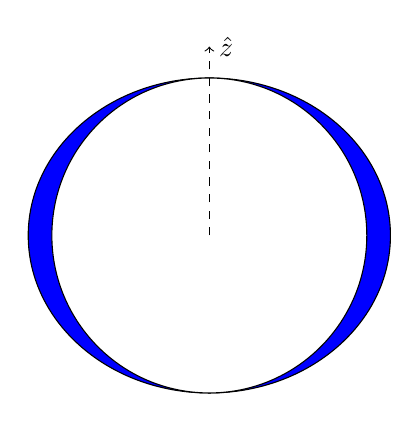
\begin{tikzpicture}
\filldraw [draw=black,fill=blue] (0,0) ellipse (2.3 and 2);
\filldraw [draw=black,fill=white] (0,0) circle (2);
\draw [dashed, ->] (0,0) -- (0,2.4) node[right] {$\hat{\bm{z}}$};
\end{tikzpicture}
\caption{Geopotential ocean surface relative to a spherical Earth.}
\label{fig:oblate}
\end{center}
\end{figure}

Imagine a spherical earth. At sea level, the polar radius is 21.4km smaller
than the equatorial radius: see figure~\ref{fig:oblate}. In reality, the
surface of the Earth is also very close to a geopotential surface. Hence
\emph{geopotential coordinates} are very useful for planetary scale motion.

\subsection{Local Cartesian coordinates}
For small motions, it is much more convenient to define \emph{local Cartesian
coordinates} (figure~\ref{fig:lcc}).
\begin{figure}
	\begin{center}
	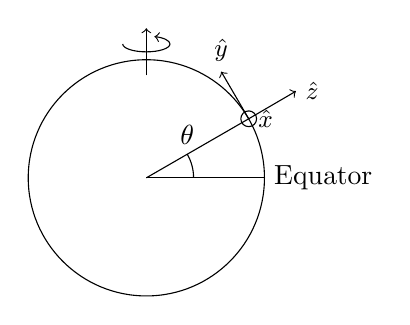
\begin{tikzpicture}
		\draw (0,0) circle (1.5);
		\draw (0,0) -- (1.5, 0) node[right] {Equator};
		\draw (0,0) -- (1.3, 0.75);
		\draw (0.6,0) arc (0:30:0.6) node[anchor = south] {$\theta$};
		\draw[->] (0,1.3) -- (0, 1.9);
		\draw[->] (0, 1.7) [partial ellipse = -180:70:0.3 and 0.1];
		\draw[->] (1.3, 0.75) -- (1.9,1.1) node[right] {\small $\hat{\bm{z}}$};
		\draw[->] (1.3, 0.75) -- (1.3 - 0.35, 0.75 + 0.6) node[above] {\small
		$\hat{\bm{y}}$};
		\draw (1.3, 0.75) circle (0.1) node[right] {\small $\hat{\bm{x}}$};
	\end{tikzpicture}
	\caption{Local Cartesian coordinates}
	\label{fig:lcc}
	\end{center}
\end{figure}

In this coordinate system $\bm{\Omega} = (0, \Omega \cos \theta, \Omega \sin
\theta)$. Hence if $\bm{u} = (u, v, w)$ then
\begin{equation}
	\begin{aligned}
		2 \bm{\Omega} \times \bm{u} &= (2\Omega w \cos \theta - 2 \Omega v \sin
		\theta, 2 \Omega u \sin \theta, -2\Omega u \cos \theta) \\
		&= (-fv + f^* w, fu - f^* u)
	\end{aligned}
\end{equation}
where $f \equiv 2 \Omega \sin \theta$ is the \emph{Coriolis parameter} and
$f^* \equiv 2 \Omega \cos \theta$.

\begin{eg}
	In Cambridge, $\theta = 52.1^{\circ} N$ so
	\begin{equation}
		\begin{aligned}
			f &= 2 \Omega \sin \theta \\
			  &= 2 \cdot \frac{2\pi}{3600 \cdot 24} \cdot 0.79 s^{-1} \\
			  &\approx 1.14 \times 10^{-4} s^{-1}
		\end{aligned}
	\end{equation}
	At mid-latitudes, $f \sim 10^{-4}$ is a good approximation.
\end{eg}

We can simplify the Coriolis acceleration expression; often $f^* w \ll f v$
and $f^* u \ll g$. Hence
\begin{equation}
	2 \bm{\Omega} \times \bm{u} \approx (-fv, fu, 0) = f \hat{\bm{z}} \times
	\bm{u}
\end{equation}

This is the \emph{traditional approximation}. This is \emph{not} always a good
approximation, particularly at intermediate scales.

\subsection{Scale analysis.}
Define characteristic scales for length $L$, time $T$, and velocity $U$.
Non-dimensional variables are denoted with a superscript star: $\bm{u}^* =
\bm{u}/U$, etc.

Using these scalings with $\bm{F} = \nu \nabla^2 \bm{u}$ we have
\begin{equation}
	\frac{U}{T} \frac{\partial \bm{u}^*}{\partial t^*} + \frac{U^2}{L}
	\bm{u}^* \cdot \nabla^* \bm{u}^* + fU \hat{\bm{z}} \times \bm{u}^* =
	-\frac{1}{\rho} \nabla \left(p + \rho \Phi\right) + \frac{\nu U}{L^2} \nabla_*^2
		\bm{u}^*
\end{equation}

Dividing through by $fU$ leaves the Coriolis acceleration term $\text{ord}(1)$ with
other terms scaled relatively.
\begin{equation}
	\frac{1}{fT} \frac{\partial \bm{u}^*}{\partial t^*} + \text{Ro}	\bm{u}^*
	\cdot \nabla^* \bm{u}^* + \hat{\bm{z}} \times \bm{u}^* =
	-\frac{1}{\rho f U} \nabla \left(p + \rho \Phi\right) + \text{E} \nabla_*^2
		\bm{u}^*
\end{equation}
where $\text{Ro} \equiv \frac{U}{fL}$ is the \emph{Rossby number} and
$\text{E} \equiv \frac{\nu}{fL^2}$ is the \emph{Ekman number}.

\begin{eg}
	For an atmospheric storm, $U \sim 10 m s^{-1}, L \sim 1000 km, f \sim
	10^{-4} s^{-1}$. Thus $\text{Ro} \sim 0.1, \text{E} \sim 10^{-13}$.
\end{eg}

\lecture{14/10/2020}
Further, if $T = L/U$, then $\text{Ro} = U/fL = 1/fT$. For small \Ro, \Ek, 
on surfaces of constant $\Phi$, $f \hat{\bm{z}} \times \bm{u} \approx
-\frac{1}{\rho}\nabla p$.  This is \emph{geostrophic balance}. In components,
we have
\begin{equation}
	\begin{aligned}
		-fv &= -\frac{1}{\rho}\frac{\partial p}{\partial x} \\
		fu &= -\frac{1}{\rho}\frac{\partial p}{\partial y}
	\end{aligned}
\end{equation}
The equations of geostrophic balance can be arranged to give the horizontal
velocity:
$\bm{u}_H$
\begin{equation}
	\bm{u}_H \equiv (u,v) = \frac{1}{\rho f} \hat{\bm{z}} \times \nabla p
\end{equation}

Horizontal velocity is perpendicular to $\nabla p$ and hence parallel to
isobars (lines of constant $p$), i.e. pressure acts like a streamfunction (see
figure~\ref{fig:isobars}).

\begin{figure}
	\centering
	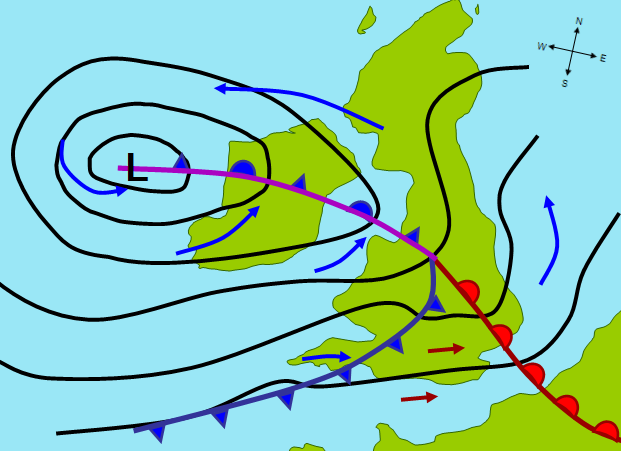
\includegraphics[width=0.4\textwidth]{isobars.png}
	\caption{Lines of constant pressure $p$ act as streamlines for the
	horizontal flow.}
	\label{fig:isobars}.
\end{figure}

In the Northern Hemisphere, air moves clockwise around high $p$ and
anticlockwise around low $p$. A \emph{cyclonic} rotation is in the same sense
as $\bm{\Omega}$, \emph{anticyclonic} in the opposite sense as $\bm{\Omega}$.

\subsection{Taylor-Proudman Theorem}
Consider an incompressible, ideal fluid in geostrophic balance (small \Ro,
\Ek)
\begin{align}
	\nabla \cdot \bm{u} &= 0\\
	2 \bm{\Omega} \times \bm{u} &= -\frac{1}{\rho}\nabla p \label{tpt}
\end{align}

Taking the curl of \eqref{tpt} we have
\begin{equation}
	\begin{aligned}
		\nabla \times \left( \bm{\Omega} \times \bm{u}\right) &= \vare_{ijk}
		\partial_j \vare_{klm} \Omega_l u_m \\
		&= \vare_{kij} \vare_{klm} \Omega_l \partial_j u_m \\
		&= \left(\delta_{il} \delta_{jm} - \delta_{im} \delta_{jl}\right)
		\Omega_l \partial_j u_m \\
		&= \Omega_i \partial_j u_j - \Omega_j \partial_j u_i
	\end{aligned}
\end{equation}

The first term is $0$ by incompressibility. Thus
\begin{equation}
	-\nabla \times \left(\bm{\Omega} \times \bm{u}\right) = \bm{\Omega} \cdot
	\nabla \bm{u} = 0
\end{equation}

For $\bm{\Omega} = (0, 0, \Omega)$, this implies $\frac{\partial w}{\partial
z} = 0$. If $w = 0$ on some horizontal surface (e.g. ground) then $w=0$
everywhere. 

Also, $u_x + v_y = 0$, i.e. horizontal velocity is non-divergent in
geostrophic balance. Fluid moves in `columns' parallel to $\bm{\Omega}$,
called \emph{Taylor columns}.

\section{Departures from geostrophy}
Consider an incompressible, rotating fluid with constant density $\rho_0$ with
angular velocity $\bm{\Omega} = (0, 0, f/2)$. Assume small ampltiude motions
(i.e. $\abs{\bm{u}}^2 \ll \abs{\bm{u}}$), i.e. neglect $\bm{u}\cdot \nabla
\bm{u}$ and $\nu \nabla^2 \bm{u}$. From \eqref{nsrot},

\begin{align}
	u_t - fv &= -\frac{p_x}{\rho_0} \label{nsrot1} \\
	v_t + fu &= -\frac{p_y}{\rho_0} \label{nsrot2}\\
	w_t &= -\frac{p_z}{\rho_0} \label{nsrot3}\\
	u_x + v_y + w_z &= 0 \label{nsrot4}
\end{align}

We will eliminate variables in favour of $p$.
\begin{equation}
	\begin{aligned}
		\nabla \cdot \left( \eqref{nsrot1} - \eqref{nsrot3}\right) &\implies
\nabla^2 p = \rho_0 f\left(v_x - u_y\right) \\
\partial_x \eqref{nsrot2} - \partial_y \eqref{nsrot1} \& \eqref{nsrot4}
&\implies (v_x-u_y)_t = fw_z \\
\end{aligned}
\end{equation}

Combining these and using \eqref{nsrot3} we have
\begin{equation}
	\nabla^2 p_{tt} + f^2 p_{zz} = 0
\end{equation}
which is a wave equation for $p$. Seek plane wave solutions with ansatz 
\begin{equation}
	p = \hat{p}e^{i\left(kx + ly + mz-\omega t\right)}
\end{equation}
and dispersion relation
\begin{equation}
	\omega^2 = \frac{f^2 m^2}{k^2+l^2+m^2} = f^2 \sin^2 \theta
\end{equation}

\begin{center}
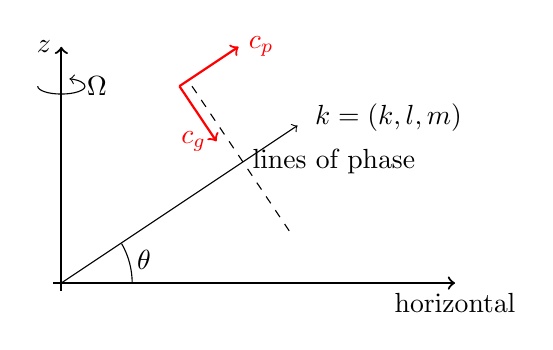
\begin{tikzpicture}
	\draw[->,thick] (-0.1,0) -- (5,0) node[below]{horizontal};
	\draw[->,thick] (0,-0.1) -- (0,3) node[left]{$z$};
	\draw[->] (0, 2.5) [partial ellipse = -180:70:0.3 and 0.1];
	\draw (0.2,2.5) node[right] {$\bm{\Omega}$};
	\draw[->] (0,0) -- (3, 2);
	\draw (3.1, 2.1) node[right] {$\bm{k} = (k, l, m)$};
	\draw (0.9,0) arc (0:30:1);
	\draw (1.05,0.3) node {$\theta$};
	\draw[dashed] (1.66, 2.5) -- (2.95,0.58) node[midway,right] {lines of phase};
	\draw[->,thick, red] (1.5, 2.5) -- (2.25, 3) node[right] {$\bm{c}_p$};
	\draw[->,thick, red] (1.5,2.5) -- (1.97, 1.8) node[left] {$\bm{c}_g$};
\end{tikzpicture}
\end{center}

This is the dispersion relation for rotating internal waves. They have phase
speed $\bm{c}_p = w/\bm{k}$ and group velocity 
\begin{equation}
	\bm{c}_g = \frac{\partial w}{\partial \bm{k}} = \pm f \frac{(-km, -lm, k^2
		+ l^2)}{\abs{\bm{k}}^{3/2}}
\end{equation}
Note that $\bm{c}_p\cdot\bm{c}_g = 0$. Also note $\abs{\omega} \le \abs{f}$.

\lecture{16/10/2020}
\subsection{Inertial (free) oscillations}
Assume $\nabla p = \bm{0}$.  The $x$ and $y$ components of geostrophic balance
\eqref{nsrot1}, \eqref{nsrot2} give
\begin{equation}
	u_{tt} + f^2 u = 0
\end{equation}
Thus $u = U \sin ft$ where $f$ is the \emph{inertial frequency}. Similarly, we
have $v = U \cos ft$. For a particle with position $(x_p, y_p)$ floating on an
ocean surface $z=0$ moving with the fluid velocity, we have
\begin{equation}
	\begin{aligned}
		\frac{\diffd x_p}{\diffd t} = u &\implies x_p = -\frac{U}{f} \cos ft +
		x_0 \\
		\frac{\diffd y_p}{\diffd t} = v &\implies y_p = -\frac{U}{f} \sin ft +
		y_0
	\end{aligned}
\end{equation}

Thus the motion of fluid particles describes describes \emph{inertial circles}
with radius $\frac{2U}{f}$.

\subsection{Ekman layer}
Look for a \emph{steady} ocean response to a constant wind stress
$\bm{\tau}_w$. Use local Cartesian coordinates and make the following assumptions:
\begin{enumerate}
	\item Steady, i.e. $\partial_t \equiv 0$
	\item Neglect horizontal variations, i.e. $\partial_x = \partial_y = 0$
	\item Neglect surface waves, i.e. $w(z=0) = 0$
	\item No flow in deep ocean, i.e. $\lim_{z \to -\infty} \bm{u} = \bm{0}$
	\item Constant density $\rho$
	\item Traditional approximation
\end{enumerate}

Continuity (incompressibility) says $u_x + v_y + w_z = 0$. Assumptions $2$ and
$3$ then imply $w = 0$ everywhere. The horizontal momentum equations are
\begin{align}
	-fv &= \nu u_{zz} \label{hmom1} \\
	fu &= \nu v_{zz} \label{hmom2}
\end{align}
Define the \emph{complex velocity} $\mathcal{V} \equiv u+iv$. Then
\begin{equation}
	\mathcal{V}_{zz} = \frac{if}{\nu} \mathcal{V} \label{compvel}
\end{equation}

Without loss of generality, assume $\bm{\tau}_w$ is aligned with the $x$-axis:
$\bm{\tau}_w = (\tau_w, 0) = (\rho \nu u_z, 0)$. Boundary conditions for
\eqref{compvel} are
\begin{equation}
	\begin{aligned}
		\mathcal{V}_z &= \left( \frac{\tau_w}{\rho \nu}, 0\right) \hspace{1em}
		\text{at} \, \, z = 0 \\
		\mathcal{V} &= (0,0) \hspace{1em} \text{as}\,\, z \to -\infty
	\end{aligned}
\end{equation}

Thus $\mathcal{V} = Ae^{(1+i)z/\delta}$ where $\delta = \sqrt{\frac{2\nu}{f}},
A = \frac{\tau_w \delta (1-i)}{2 \rho \nu}$. In terms of the velocity
components, we have
\begin{equation}
	\begin{aligned}
		u &= \frac{\tau_w}{\rho \sqrt{\nu f}} e^{z/\delta} \cos \left(
		-\frac{z}{\delta} + \frac{\pi}{4}\right) \\
		v &= -\frac{\tau_w}{\rho \sqrt{\nu f}} e^{z/\delta} \sin \left(
		-\frac{z}{\delta} + \frac{\pi}{4}\right) \\
	\end{aligned}
\end{equation}

A top view of the ocean shows an \emph{Ekman spiral}: see
figure~\ref{fig:ekman}.
\begin{figure}
	\centering
	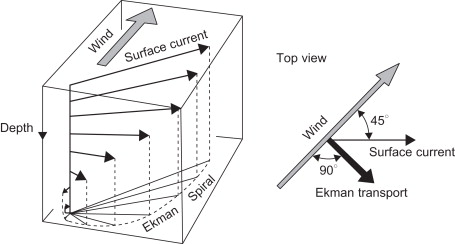
\includegraphics[width=0.5\textwidth]{ekman_spiral.jpg}
	\caption{Ekman spiral.}
	\label{fig:ekman}
\end{figure}

\subsection{Ekman transport}
Integrate the horizontal momentum equations \eqref{hmom1},\eqref{hmom2} to the
base of the Ekman layer where $\nu \bm{u}_z \approx 0$ at $z=-h$. Since $\nu
\bm{u}_z (z=0) = (\tau_w/\rho, 0)$, the \emph{Ekman transport} $\bm{U}_T$ is
\begin{equation}
	\begin{aligned}
		U_T &\equiv \int_{-h}^0 u \, \diffd z = 0 \\
		V_T &\equiv \int_{-h}^0 v \, \diffd z = -\frac{\tau_w}{\rho f}
	\end{aligned}
\end{equation}

This is the net transport of fluid in the Ekman layer and is oriented
$90^{\circ}$ to the right of the applied wind shear stress (in the Northern
Hemisphere).

\subsection{Ekman pumping}
Consider a wind stress $\tau_w(y)$ that varies over large scales. Then from
incompressibility
\begin{equation}
	\int_{-h}^0 w_z \, \diffd z = -\int_{-h}^0 u_x \, \diffd z - \int_{-h}^0
	v_y \, \diffd z
\end{equation}

Thus for $h$ constant, 
\begin{equation}-w(z=-h) = -\frac{\partial V_T}{\partial y} =
\frac{\partial}{\partial y}\left( \frac{\tau_w}{\rho f}\right)
\end{equation}

In general we have
\begin{equation}
	w(z=-h) = \hat{\bm{z}} \cdot \nabla \times \frac{\bm{\tau}_w}{\rho f}
\end{equation}

\lecture{19/10/20}
\section{Rotating shallow water equations}
Consider a thin layer of fluid with constant density $\rho$. Define
characteristic scales
\begin{itemize}
	\item length $L = \text{horiz.}, H = \text{vert.}$
	\item velocity $U$
	\item time $T$
	\item pressure $P$
\end{itemize}
such that $\partial_x, \partial_y \sim \frac{1}{L}, \partial_z \sim
\frac{1}{H}$. Define the \emph{aspect ratio} $\delta \equiv H/L$. We will
assume $\delta \ll 1$. From continuity (incompressibility) we have
\begin{equation}
	\begin{aligned}
		\frac{\partial w}{\partial z} &= -\frac{\partial u}{\partial x} -
		\frac{\partial v}{\partial y}  \\
		\implies \frac{w}{H} &= \mathcal{O}(U/L) \\
		\implies w &= \mathcal{O}(\delta U)
	\end{aligned}
\end{equation}

Using the traditional approximation and assuming the fluid is inviscid, the
$x$-momentum equation
\begin{align}
	&\frac{\partial u}{\partial t} &&+ u \frac{\partial u}{\partial x} &&+v
	\frac{\partial u}{\partial y} &&+ w\frac{\partial u}{\partial z} &&- fv &&=
						&&-\frac{1}{\rho} \frac{\partial p}{\partial x}
	\label{eq:swxmom}\\
	\text{scaling:}\hspace{1em} &\frac{U}{T} &&\frac{U^2}{L} && \frac{U^2}{L}
					&&\frac{wU}{H} &&fU &&= &&\frac{P}{\rho L}
\end{align}

Thus if $p_x$ appears at leading order then
\begin{equation}
	P \sim \rho U \max(L/T, U, fL)
\end{equation}

Similarly the $z$-momentum equation and its scalings are
\begin{align}
	&\frac{\partial w}{\partial t} &&+ u \frac{\partial w}{\partial x} &&+v
	\frac{\partial w}{\partial y} &&+ w\frac{\partial w}{\partial z} &&=
						&&-\frac{1}{\rho} \frac{\partial p}{\partial x} - g
	\label{eq:swzmom} \\
	\text{scaling:}\hspace{1em} &\frac{w}{T} &&\frac{Uw}{L} && \frac{Uw}{L}
					&&\frac{w^2}{H} &&= &&\frac{P}{\rho H}
\end{align}

Hence $\frac{\diffD w}{\diffD t} \sim \max(\frac{w}{T}, \frac{Uw}{L})$. Comparing with the
pressure term, we have
\begin{align}
	\frac{\frac{\diffD w}{\diffD t}}{\frac{1}{\rho}\frac{\partial p}{\partial
		z}} &\sim \frac{\max(\frac{w}{T},
		\frac{Uw}{L})}{\frac{U}{H}\max(\frac{L}{T}, \frac{U}{L}, f)}\\
		&\sim \delta^2
		\frac{\max(\frac{1}{T},\frac{U}{L})}{\max(\frac{1}{T},\frac{U}{L},f)}
\end{align}

Therefore to $\mathcal{O}(\delta^2)$ we have \emph{hydrostatic balance}. To
this order, \eqref{eq:swzmom} becomes
\begin{equation}
	\frac{\partial p}{\partial z} - \rho g \implies p = \rho g (\eta - z)
\end{equation}
assuming $p = 0$ at $z = \eta(x,y,t)$. Similarly, we have $\frac{1}{\rho} p_x
= g \eta_x$ and $\frac{1}{\rho} p_y = g \eta_y$. Hence horizontal acceleration
(i.e. the LHS of \eqref{eq:swxmom}) is independent of $z$. Motivated by this,
we \emph{assume} that horizontal velocity is also independent of $z$. For $\Ro
\ll 1$, this follows from the Tayor-Proudman theorem.

Re-writing \eqref{eq:swxmom} with these results we have
\begin{align}
	u_t + u u_x + v u_y -fv &= -g \eta_x \label{eq:swx}\\
	v_t + u v_x + v v_y + fu &= -g \eta_y \label{eq:swy}
\end{align}
since $u_z = v_z = 0$ by assumption. Integrating the continuity equation gives
\begin{equation}
	w = -z(u_x + v_y) + A(x,y,t)
\end{equation}
where $A$ is to be determined by the boundary conditions. Requiring no normal
flow at $z = -H_0 + h_b$ is imposed by $\bm{u}\cdot\hat{\bm{n}} = 0$ where
$\bm{n} = \nabla(z-h_b)$. Thus
\begin{equation}
	-u\frac{\partial h_b}{\partial x} -v \frac{\partial h_b}{\partial y} + w = 0
\end{equation}

Hence
\begin{equation}
	A(x,y,t) = u \frac{\partial h_b}{\partial x} + v \frac{\partial
	h_b}{\partial y} + (-H_0 + h_b) (u_x+v_y)
\end{equation}

The kinematic boundary condition at $z = \eta$ is $\frac{\diffD \eta}{\diffD
t} = w$ which may be written as
\begin{equation}
	\eta_t + u \eta_x + v \eta_y - w = 0
\end{equation}
where $w = -\eta(u_x+v_y) + u \frac{\partial h_b}{\partial x} + v
\frac{\partial h_b}{\partial y} + (-H_0 + h_b)(u_x+v_y)$. Combining these
boundary conditions gives
\begin{equation}
	\eta_t + \left[ (H_0-h_b+\eta)u\right]_x + \left[ (H_0-h_b+\eta)v\right]_y
	= 0 \label{eq:swcon}
\end{equation}
If $H \equiv H_0 - h_b + \eta$ is the total depth of the fluid, then since
$H_t = \eta_t$,
\begin{equation}
	H_t + (uH)_x + (vH)_y = 0 \label{eq:swcon2}
\end{equation}
which is a statement of the conservation of volume (equivalently mass, since
$\rho$ is constant). Equations \eqref{eq:swx}, \eqref{eq:swy}, and
\eqref{eq:swcon} are the \emph{rotating shallow water} (SW) equations.

\subsection{Potential vorticity (PV)}
Denote the vertical vorticity by $\zeta = v_x - u_y$. Consider $\partial_x
\eqref{eq:swy} - \partial_y \eqref{eq:swx}$, which gives
\begin{equation}
	\zeta_t +u\zeta_x + v\zeta_y + v f_y = -(\zeta + f)(u_x+v_y)
\end{equation}
Now from conservation of volume \eqref{eq:swcon2},
\begin{equation} 
	u_x + v_y = -\frac{1}{H} \frac{\diffD H}{\diffD t}
\end{equation}
Combining these relates the material derivative of $\zeta$ and $H$ by
\begin{equation}
	\frac{\diffD \zeta}{\diffD t} = \frac{\zeta + f}{H} \frac{\diffD H}{\diffD
	t} \implies \frac{\diffD}{\diffD t}\left(\frac{\zeta + f}{H}\right) = 0
	\label{eq:PV}
\end{equation}

Let $q \equiv \frac{\zeta + f}{H}$, the \emph{shallow water potential
vorticity} (SWPV). SWPV is conserved following fluid motion. We call $\zeta$
the \emph{relative vorticity} and $f$ the \emph{planetary vorticity}. $\zeta$
and $f$ will change as a fluid moves to conserve SWPV (changing $f$) and
angular momentum (changing depth).

\begin{center}
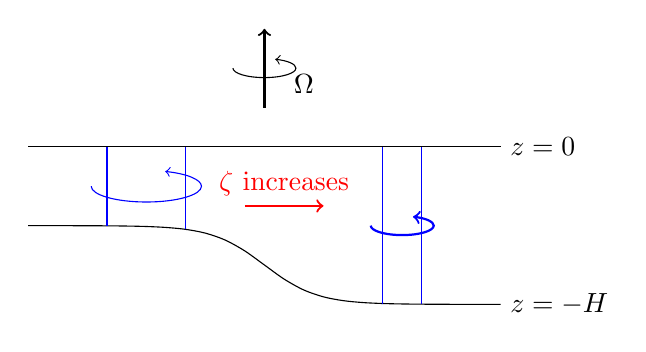
\begin{tikzpicture}
	\draw[thick,->] (0,2.5) -- (0, 3.5);
	\draw[->] (0, 3) [partial ellipse = -180:70:0.4 and 0.12];
	\draw (0.5, 2.8) node {$\bm{\Omega}$};
	\draw[smooth,domain=-3:3] plot({\x}, {1/(1+exp(3*\x))});
	\draw[smooth,domain=-3:3] plot({\x}, {2});
	\draw (3,2) node[right] {$z=0$};
	\draw (3,0) node[right] {$z=-H$};
	\draw[blue] (-2,0.998) -- (-2,2);
	\draw[blue] (-1,0.953) -- (-1,2);
	\draw[blue] (1.5,0.011) -- (1.5, 2);
	\draw[blue] (2,0.002) -- (2,2);
	\draw[thick,blue,->] (1.75, 1) [partial ellipse = -180:70:0.4 and 0.12];
	\draw[blue,->] (-1.5, 1.5) [partial ellipse = -180:70:0.7 and 0.2];
	\draw[red, thick, ->] (-0.25,1.25) -- (0.75, 1.25) node[midway,above]
		{$\zeta$ increases};
\end{tikzpicture}
\qquad
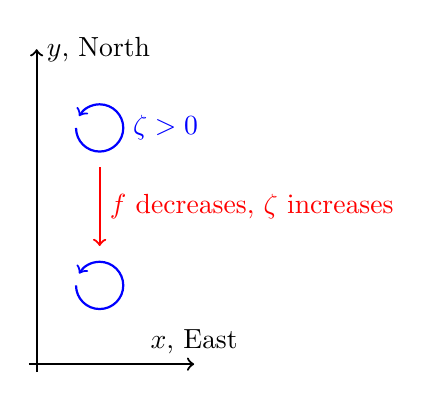
\begin{tikzpicture}
	\draw[thick,->] (-0.1,0) -- (2, 0) node[above] {$x$, East};
	\draw[thick,->] (0,-0.1) -- (0, 4) node[right] {$y$, North};
	\draw[thick,blue,->] (0.5, 3) arc(-180:150:0.3);
	\draw[thick,blue,->] (0.5, 1) arc(-180:150:0.3);
	\draw[thick,red,->] (0.8, 2.5) -- (0.8, 1.5) node[midway,right] {$f$
		decreases, $\zeta$ increases};
	\draw[blue] (1.1, 3) node[right] {$\zeta > 0$};
\end{tikzpicture}
\end{center}


\end{document}
